%*****************************************
\chapter{Stand der Forschung}\label{ch:relatedWork}
%*****************************************

\section{Health IT Ontology}

\subsection{Allgemein}

Die Welt der medizinischen Informatik umfasst eine Vielzahl an Begriffe, Werkzeuge und Prozesse. 
Dies führt beim Vergleich von IT-Komponenten im Gesundheitswesen, aufgrund von diversen Terminologien zu Schwierigkeiten. 
Aus diesem Grund wurde \ac{HITO} ins Leben gerufen.
\ac{HITO} ermöglicht eine systematische Beschreibung von Anwendungssystemen und Softwareprodukten innerhalb von Krankenhausinformationssystemen.
So unterstützt\ac{HITO} das Management, die Weiterbildung und die Lehre im Bereich der medizinischen Informatik.

\subsection{Use Cases}

Use Cases beschreiben Situationen in denen ein Produkt genutzt werden kann.
Im folgenden werden die Use Cases für HITO erläutert. \newline

\textbf{Use Case 1}: Mitarbeiter des Informationsmanagements möchten in einer \ac{KIS} Strategie-Besprechung, die existierenden Komponente des \ac{KIS} für alle Teilnehmer verständlich erklären.
Im Idealfall verfügen alle Teilnehmer über die selbe Terminologie.
Das ist aber in der Realität anders, da die Teilnehmer aufgrund der individuellen Spezialisierungen und Fachbereiche jeweils unterschiedliche Terminologien verwenden. \newline

\textbf{Use Case 2}:  Mitarbeiter des Informationsmanagements möchten ein neues Softwareprodukt für das Krankenhausinformationssystem auswählen.
In dieser Situation entstehen Fragen wie zum Beispiel: "Wie wählt man Software-Produkte für das \ac{KIS} von dem Markt aus?" oder \enquote{Welche andere Organisationen haben ähnliche Anwendungssysteme im Rahmen ihres \ac{KIS}}
In diesem Fall steht man vor der Herausforderung, dass Software-Hersteller unterschiedliche Terminologien für die Beschreibung ihrer Software-Produkte nutzen.
Somit lassen sich diese Beschreibungen nicht vergleichen. \newline

\textbf{Use Case 3}: Mitarbeiter des Informationsmanagements, die über geringe finanzielle Ressourcen verfügen, möchten ein Anwendungssystem installieren, das ein kostenloses oder Open-Source Software-Produkt ist.
In diesem Fall, möchten sich Mitarbeiter über die verfügbaren kostenlose/open-source Produkte und deren Eigenschaften informieren.
Das Problem bei diesem Use-Case besteht darin, dass kostenlose/open-source Produkte nicht so gut vermarktet sind wie kommerzielle Software-Produkte. 
In diesem Fall stolpert(besseres Wort finden) man zusätzlich auch, über die im Use Case 2 beschriebene Herausforderung. \newline

\textbf{Use Case 4}: Mitarbeiter des Informationsmanagements, möchten sich bezüglich eines KIS-Anwendungssystems oder eines Software-Produkts evidenzbasierte Daten anschauen.  \newline

\textbf{Use Case 5}: Mitarbeiter des Informationsmanagements möchten neue Mitarbeiter einstellen oder das existierende Personal weiterbilden.
Dafür muss eine Liste an Anforderungen zusammengestellt werden.
In diesem Fall kommen Fragen wie zum Beispiel: \enquote{Welche Ausbildungen werden für bestimmte Software Produkte angeboten?} oder \enquote{Welche Spezialisten mit bestimmte Kompetenzen sind aktuell auf dem Arbeitsmarkt verfügbar?}.
Hier besteht das Problem, dass diese Art von Informationen nicht systematisch aufbereitet sind, sondern nur als Freitext verfügbar sind.\newline

\subsection{Aufbau}

Das \ac{HITO}-Metamodell stellt den Aufbau der Ontologie dar. 
Das Metamodell enthält, die in der Ontologie enthaltenen Klassen und Relationen.
Die Abbildung \ref{fig:metamodel} stellt das Metamodell von HITO dar und die Tabelle \ref{table:hito_klassen} enthält alle Klassen von HITO mit einer Beschreibung.. 

\begin{sidewaysfigure}[h]
    	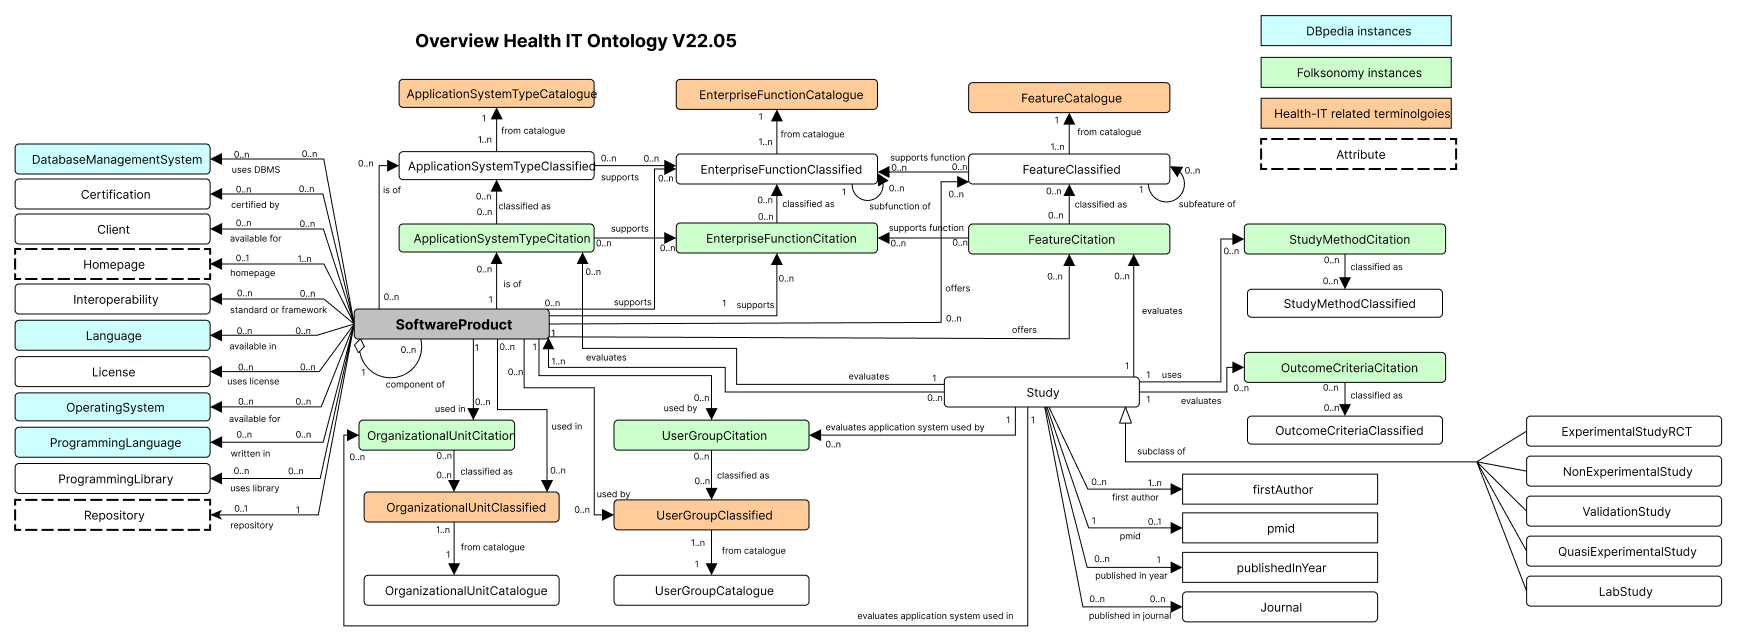
\includegraphics[width=\textwidth]{Images/hito_metamodell}
   	\caption{HITO-Metamodell}
   	\label{fig:metamodel}
\end{sidewaysfigure}

\clearpage

\begin{longtable}{ | p{4,5 cm} | p{7 cm} | }
\hline
\textbf{Klasse} & \textbf{Definiftion} \\ \hline
\endhead
Application System Type Catalogue & Eine Sammlung von klassifizierten Anwendungssystemen. \\
\hline
Application System Type Citation & Der Begriff, den ein Autor für das Anwendungssystem verwendet, das in der Studie bewertet wird. \\
\hline
Application System Type Classified & Der Begriff für ein Anwendungssystem, der in der Klassifizierung von Anwendungssystemen verwendet wird. \\
\hline
Catalogue & Eine Sammlung von klassifizierten Begriffe der gleichen Art aus der gleichen Quelle. \\
\hline
Certification & Zertifikat eines Softwareprodukts zur Bewertung der Einhaltung der Normen des Qualitätsmanagements. \\
\hline
Citation & Beschreibung eines Softwareprodukts in natürlicher Sprache anhand der Produktdokumentation, z. B. einer Webseite. \\
\hline
Classified & Klassifiziert einen Eintrag eines Katalogs, wie z.B. ein Merkmal oder eine Unternehmensfunktion. \\
\hline
Client & Die Art der Hardware- und Softwareumgebung, auf der ein Softwareprodukt ausgeführt werden kann. \\
\hline
Database System & Database Management System, wie z.B. MySql oder PostegreSql.\\
\hline
Enterprise Function Citation & Das natürlichsprachliche Zitat einer Unternehmensfunktion beschreibt, was die handelnden Menschen oder Maschinen in einem bestimmten Unternehmen zu tun haben, um zu dessen Aufgabe oder Zielen beizutragen. Eine Unternehmensfunktion ist eine Richtlinie in einer Institution, wie Daten über Entitätstypen zu interpretieren sind und dann Daten über Entitätstypen als Folge dieser Interpretation zu aktualisieren sind. Das Zitat ist ein Begriff, den ein Autor verwendet, um die Unternehmensfunktion zu beschreiben, die durch ein Anwendungssystem unterstützt wird. \\
\hline
Enterprise Function Classified & Der Begriff für eine Unternehmensfunktion, der in der Klassifizierung von Unternehmensfunktionen verwendet wird. Es ist ein klassifizierter Begriff im Sinne unserer Definition, der zu einer Klassifikation gehört. \\
\hline
Experimental Study RCT &  Experimentelle Studie mit randomisiertem Kontrollversuch. \\
\hline
Feature Catalogue & Eine Sammlung von klassifizierten Softwarefunktionen. \\
\hline
Feature Citation & Features sind vom Softwareprodukt des Anwendungssystems angebotene Funktionalitäten, die direkt zur Erfüllung einer oder mehrerer Funktionen beitragen. Je feiner die Granularität einer Funktion formuliert ist, desto größer ist die Wahrscheinlichkeit, dass die Funktion semantisch mit einem Feature einer Anwendungskomponente übereinstimmt. \\
\hline
Feature Classified & Der zusammenfassende Begriff eines Merkmals, der in Katalogen verwendet wird. Es ist ein klassifizierter Begriff nach unserer Definition, der zu einer Klassifikation gehört.  \\
\hline
Function Catalogue & Eine Sammlung von klassifizierten Unternehmensfunktionen. \\
\hline
Interoperability & Interoperabilität ist im Allgemeinen die Fähigkeit von zwei oder mehr Komponenten, Informationen auszutauschen und die ausgetauschten Informationen zu nutzen. Normen bieten eine gemeinsame Sprache und eine Reihe gemeinsamer Erwartungen, die die Interoperabilität zwischen Systemen und/oder Geräten ermöglichen. Um Informationen über eine Person nahtlos zu verarbeiten und die Gesamtkoordination und -bereitstellung der Gesundheitsversorgung zu verbessern, ermöglichen Normen Ärzten, Labors, Krankenhäusern, Apotheken und Patienten den Austausch von Daten unabhängig von der Anwendung oder dem Marktanbieter. \\
\hline
Journal & Wissenschaftliche Zeitschrift. \\
\hline
Lab Study & Laborstudie. \\
\hline
Language & Sprache. \\
\hline
Non Experimental Study & Nicht-experimentelle Studie. \\
\hline
Operating System & Die DBpedia-Instanzen wurden unter dieser HITO-Klasse gebündelt, da DBpedia nicht gut geeignet war. \\
\hline
Organizational Unit Catalogue & Eine Sammlung von klassifizierten Organisationseinheiten. \\
\hline
Organizational Unit Citation & Der Begriff, den ein Autor für die Organisationseinheit verwendet, in der die Auswertung des Anwendungssystems stattfindet. \\
\hline
Organizational Unit Classified & Klassifizierter Katalogeintrag einer Organisationseinheit. Das SNOMED CT-Konzept von SNOMED International. \\
\hline
Outcome Criteria Citation & Der Begriff, den ein Autor für die Ergebniskriterien der Bewertungsstudie verwendet. \\
\hline
Outcome Criteria Classified & Klassifizierter Katalogeintrag eines Ergebniskriteriums. \\
\hline
PMID & The PMID extracted from PubMed for each study. \\
\hline
Prgramming Language & Programmiersprache. \\ 
\hline
Programming Library & Eine Programmierbibliothek ist eine Sammlung von wiederverwendbarem Code. \\
\hline
Quasi Experimental Study & Empirische Interventionsstudie ohne Randomisierung. \\
\hline
Software Product & Ein Softwareprodukt ist ein erworbenes oder selbst entwickeltes Softwareprgramm, das auf einem Computersystem installiert werden kann. \\
\hline
Software Product Installation & Also known as Computer-based application component. Based on a software product, which is an acquired or self-developed piece of software that can be installed on a computer system. For example, the computer-based application component patient administration system stands for the installation of a software product to support enterprise functions such as patient admission and administrative discharge and final billing. \\
\hline
Study & Eine Evaluationsstudie. \\
\hline
Study Method Citation & The natural language term an author uses for a study method which is used in the evaluation study. \\
\hline
Study Method Classified & The study method, qualitative or quantitative. \\
\hline
User Group Catalogue & A collection of classified user groups. \\
\hline
User Group Citation & Der Begriff, den ein Autor für die Benutzergruppe eines Anwendungssystems verwendet. \\
\hline
User Group Classified & Das SNOMED CT-Konzept von SNOMED International. SNOMED CT - Internationaler SNOMED CT Browser [Internet]. Release: International Edition 20190131. 2019 [cited 2019 Mar 26]. Verfügbar unter: https://browser.ihtsdotools.org/? \\
\hline
Validation Study & Vergleicht die Genauigkeit einer Messung mit einer Standardmessung.\\
\hline
\caption{Klassen von HITO}
\label{table:hito_klassen}
\end{longtable}


